\documentclass[a4paper]{oblivoir}
% define the title
\author{Moon Il-chul \\ \href{mailto:icmoon@kaist.ac.kr}{icmoon@kaist.ac.kr} 
   \and Hwang Gyeong-jo
 \\ \href{mailto:hkj4276@kaist.ac.kr}{hkj4276@kaist.ac.kr} }
\setcounter{chapter}{6}
\title{Chapter 6. Training/Testing and Regularization}
\usepackage{indentfirst}
\usepackage{graphicx}
\graphicspath{ {Figure/} }
\usepackage{hyperref}
\usepackage{amsmath}
\usepackage{amssymb}
\usepackage{amsfonts}
\usepackage{dsfont}
\usepackage[]{algorithm2e}
\usepackage{chngcntr}
\counterwithin{figure}{chapter}
\setcounter{tocdepth}{2}
\setcounter{secnumdepth}{3}
\hypersetup{pdfborder={0 0 0}}
\renewcommand{\thefigure}{\thechapter-\arabic{figure}}
\renewcommand{\theequation}{\thechapter.\arabic{equation}}
\newlength\myindent
\setlength\myindent{5em}

\begin{document}
% generates the title
\maketitle
%\renewcommand{\contentsname}{목차}
\tableofcontents
%\listoftables
%\listoffigures

%슬라이드 2, 4
\section*{}
지금까지 Naive Bayes, Logistic Regression, Support Vector Machine 등 기계학습의 고전적인 Classification 방법론들을 배워보았다. 이중에서도 특히 SVM은 아직도 여러 응용 분야에서 사용되고 있고, 이를 이용한 연구 결과 등이 각종 저널에 발표되고 있다. 독자들 중에는 자신의 분야에서 이러한 도구들을 이용해보고자 하는 사람들도 있을 것이다. 하지만, 이에 앞서 위의 알고리즘들이 얼마나 좋은 성능(Performance)을 보이는지 측정하는 법을 알아야한다. 따라서 이번 단원에서는, 또한 여러 가지 성과지표(Performance Measure)들의 정의와 이들의 상관관계, 그리고 성능을 올릴 때의 근본적인 한계에 대해서 배울 것이다.

%슬라이드 3
\section{Concept of Bias and Variance}

%슬라이드 5
먼저 다음 문장을 살펴보자; ''이 Naive Bayes Classifier는 스팸 메일을 95\%의 정확도로 거를 수 있어!'' 만약 이 Classifier를 테스트한 데이터 셋이 95개의 스팸 메일과 5개의 정상 메일로 이루어져 있고, 해당 NB Classifier는 모든 메일을 스팸 메일로 분류한다면 어떨까? 분명 이 데이터 셋에 대해서 이 알고리즘은 95\%의 정확도로 메일을 분류할 것이다. 그렇다면 앞서 본 문장은 옳은 주장일까?  \\
\indent 이에 대한 답을 하기 위해서는 먼저, ''정확도(Accuracy)''라는 용어의 정의부터 확실히 해야 한다. 이후에 우리는 Precision, Recall, F-measure 등 정확도를 정의하는 여러 가지 방법에 대해 배워볼 것이다. 또한 알고리즘의 성능을 측정하기 위해 사용하는 데이터 셋의 타당성도 검사해야 한다. 예를 들어, 해당 데이터를 어디서 받아왔는지, 그 중 스팸 메일이 얼마나 들어있는지, 만약 여러 데이터 셋들이 있다면 스팸 메일의 분포에 큰 변화(Variance)가 있는지 등을 확인할 필요가 있다.

%슬라이드 6
\subsection{기계학습에서의 학습과 테스트}
기계학습에서 학습이란, Parameter(매개 변수)를 추정하는 과정 혹은 Prior Knowledge(사전 지식)와 Past Experience(과거 경험)를 이용하여 패턴을 배우는 과정이라 할 수 있다. 하지만 이러한 학습의 결과가 미래를 정확히 예측할 수 있을까? 만약 학습하는 단계에서의 데이터 셋과 테스트하는 단계에서의 데이터 셋이 다르다면 어떨까? 당연히 해당 알고리즘은 아무것도 올바르게 예측할 수 없을 것이다. 즉, 학습 대상이 되는 데이터 셋의 Domain이 변하지 않아야, 혹은 데이터 셋의 분포(Distribution)에 변화가 없어야 해당 알고리즘이 성공적인 결과를 보일 것이다. 또한, 학습을 시키려는 Target 데이터 셋이 충분한 변동성(Variance)을 보이지 않으면, 적절한 수준의 학습이 이루어지지 않을 수도 있다. \\
\indent 테스트 과정은 학습된 기계학습 알고리즘을 평가하는 과정, 다시 말해서 추정한 Parameter를 평가하는 과정이다. 이 때 평가에 사용하는 데이터(Test Dataset)와 학습에 사용된 데이터(Training Dataset) 사이에는 어떠한 연관성도 있어선 안 된다. 이를 위해서 흔히 사용하는 방법은 가지고 있는 전체 데이터를 8:2 정도의 비율로 나누어 트레이닝 데이터 8, 테스트 데이터 2 로 구분하여 진행하는 것이다. 전체 데이터가 특정 분포를 따른다면, 임의로 나눈 트레이닝 데이터와 테스트 데이터 모두 동일한 분포를 따르므로 Domain의 변화는 없다. 다음의 그림을 살펴보자.
\begin{figure}[ht]
\centering
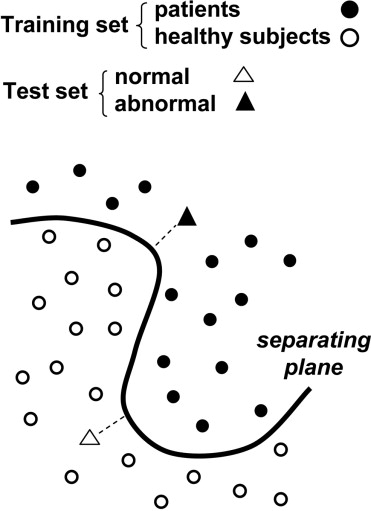
\includegraphics[scale=0.5]{Training_&_Testing.png}
\caption{Training Dataset 과 Test Dataset 의 구분 예시}
\label{Figure 6-1}
\end{figure}

\indent 위의 그림에서 전체 데이터 셋은 색칠된 도형(몸에 이상이 있는 사람)과 색칠되지 않은 도형(건강한 사람)으로 나눌 수 있다. 여기서 원 형태의 도형은 트레이닝 데이터로 구분, 삼각형 형태의 도형은 테스트 데이터로 구분하였다. 먼저 원형의 도형들을 이용하여 학습시킨 결과, 실선과 같은 결정경계(Decision Boundary)를 얻을 수 있었고, 이를 통해 2개의 삼각형 도형들을 올바르게 구분할 수 있다. 이 그림은 Outlier가 하나도 없는 이상적인 경우인데, 실제로는 그림처럼 완벽한 결정경계를 찾을 수 없을뿐만 아니라 테스트 데이터에도 잡음이 있어 100\%의 확률로 분류를 성공시킬 수 없다.

%슬라이드 7
\subsection{Over-fitting and Under-fitting}
다음의 경우를 생각해보자; 당신은 N개의 값으로 이루어진 데이터를 받았고, 기계학습 알고리즘을 학습시켜야 한다. 이를 위해 다항회귀 함수 $y=f(x)$를 학습시키고자 하는데 함수 $y$의 차수를 아직 결정하지 못했다. 물론, 비선형함수를 이용할 수도 있다. 다항함수의 차수를 변화시켰을 때, 다음 그림과 같은 상황이라면 어떻게 해야할까?
\begin{figure}[ht]
\centering
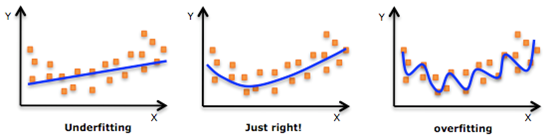
\includegraphics[scale=0.5]{Over_Under_Fitting.png}
\caption{데이터 분포와 Under-fitting, Over-fitting 의 예시}
\label{Figure 6-2}
\end{figure}

\indent 먼저 왼쪽의 선형회귀 결과를 살펴보면, 데이터 양끝의 올라가는 부분이 잘 설명되지 않음을 볼 수 있다. 함수의 차수를 지나치게 낮게 설정하면, 이렇게 데이터 분포를 적절히 설명하지 못하는 결과(Under-fitting)를 가져올 것이다. 오른쪽의 다항회귀 결과를 보면, 함수가 최소 10차 함수 쯤은 되어 보임을 알 수 있는데, 주어진 데이터 분포는 아주 잘 설명하는 것으로 보인다. 하지만 모든 데이터를 완벽하게 설명하려고(Over-fitting) 함수의 차수를 지나치게 높게 설정하면, 앞으로 주어질 데이터, 즉 테스트 데이터에 대해서는 오히려 더 큰 오차를 가질 수 있다. 이 예시에서는 가운데 그림처럼 2차 함수 형태만으로도 주어진 데이터 분포를 충분히 설명할 수 있다. 그렇다면 Over-fitting이나 Under-fitting을 피하려면 어떻게 해야 할까?

%슬라이드 8
\subsubsection{Tuning Model Complexity}
1차, 2차, $\dots$, N차 다항함수를 사용한다고 했을 때, 차수가 높은 모델을 더 복잡한(Complex) 모델이라고 한다. 그렇다면 복잡할수록 더 좋은 모델일까? 앞에서 논의한 바에 따르면 그렇지 않다. 특정 순간이 오면 모델의 복잡성(Complexity) 증가를 멈춰야 한다. 이를 좀 더 학술적으로 표현하면, ''모델의 복잡성과 데이터 셋의 일반성 사이에는 Tradeoff 가 있다.''

%슬라이드 9
\subsection{기계학습에서 오차의 요인}
기계학습에서 오차의 원인에는 두 가지 측면이 있는데, Approximation과 Generalization이 그것이다. 전자는 말그대로 기계학습 알고리즘 자체가 실제 현상을 근사하여 설명하면서 발생하는 오차이고, 후자는 트레이닝 데이터 셋의 일반성의 정도가 충분하지 않을 때, 테스트 데이터에서 잘 설명되지 않는 데이터가 입력되면 발생하는 오차이다. Approximation에 의한 오차를 $E_{in}$, Generalization에 의한 오차를 $\Omega$, 모든 측정 오차를 다 포함하는 전체 오차를 $E_{out}$라고 표기하자. 이 때 다음의 관계가 성립한다.
\begin{equation}E_{out} \leq E_{in} + \Omega \tag{6-1} \end{equation}

\indent 몇 가지 기호들을 더 정의하고 나서 다음 장으로 넘어가도록 하자.
\begin{itemize}\itemsep0pt
\item $f$: 학습시키고자 하는 목표 함수 (True function)
\item $g$: 기계학습 알고리즘을 통해 학습시킨 함수
\item $g^{(D)}$: 주어진 데이터 셋 $D$를 이용하여 학습시킨 함수 / 혹은 하나의 가설 인스턴스(Instance)
\item $D$: 관측을 통해 얻은 데이터 셋
\item $\bar{g}$: 무한 번 반복을 통해 얻은 $g^{(D)}$의 평균; 즉, $\bar{g} = E_{D}[g^{(D)}(x)]$
\end{itemize}

%슬라이드 10
\subsection{Bias and Variance}
하나의 인스턴스  $g^{(D)}$의 오차를 어떻게 표현할 수 있을까? 먼저, 다음과 같은 평균 제곱오차(Mean Squared Error; MSE)를 정의하자.
\begin{equation}E_{out}[g^{(D)}(x)] = E_{X}\left[\left(g^{(D)}(x) - f(x)\right)^{2}\right]\tag{6-2} \end{equation}
그리고, 무한 개의 데이터 셋 $D$에 대한 기댓값을 계산하자;
\begin{align}
E_{D}\left[ E_{out}[g^{(D)}(x)] \right] &= E_{D}\left[ E_{X}\left[\left(g^{(D)}(x) - f(x)\right)^{2}\right] \right] \tag{6-3} \\
&=E_{X}\left[ E_{D}\left[ \left( g^{(D)}(x) - f(x) \right)^{2} \right] \right] \tag{6-4}
\end{align}
식 6-4 에서 기댓값 괄호 안 부분을 먼저 정리하면;
\begin{align}
&E_{D}\left[ \left( g^{(D)}(x) - f(x) \right)^{2} \right] \notag \\
&= E_{D}\left[ \left( g^{(D)}(x) - \bar{g}(x) + \bar{g}(x) - f(x) \right)^{2} \right] \tag{6-5} \\
&= E_{D}\left[\left(g^{(D)}(x)-\bar{g}(x)\right)^{2}+\left(\bar{g}(x)-f(x)\right)^{2}+2\left(g^{(D)}(x)-\bar{g}(x) \right) \left(\bar{g}(x)-f(x) \right) \right] \tag{6-6}
\end{align}
\begin{align}
&= E_{D}\left[\left(g^{(D)}(x)-\bar{g}(x)\right)^{2} \right]+\left(\bar{g}(x)-f(x) \right)^{2}+E_{D}\left[2\left(g^{(D)}(x)-\bar{g}(x)\right) \left(\bar{g}(x) - f(x) \right) \right] \tag{6-7}
\end{align}

\indent 식 6-5 는 절댓값 기호를 포함한 부등식을 정리할 때와 기댓값을 계산할 때 많이 사용하는 기술인데, $\bar{g}(x) = E_{D}[g^{(D)}(x)]$ 항을 한 번 빼주고 다시 더해주는 형태로 나타낸 뒤, 식 6-6 과 같이 제곱식을 전개해주는 것이다. 그리고 식 6-7 에서 마지막 항은 다음과 같이 정리할 수 있다;
\begin{align}
E_{D}&\left[2\left(g^{(D)}(x)-\bar{g}(x)\right) \left(\bar{g}(x) - f(x) \right) \right] \notag \\
&=2\left(\bar{g}(x) - f(x) \right) E_{D}\left[\left(g^{(D)}(x)-\bar{g}(x)\right) \right] \tag{6-8} \\
&= 0 \tag{6-9}
\end{align}

\indent 이 항은 데이터 셋 $D$에 대한 기댓값을 계산하는 식이므로, $\left(\bar{g}(x)-f(x) \right)$ 부분은 기댓값 괄호 밖으로 나올 수 있고(식 6-8), 나머지 $E_{D}\left[\left(g^{(D)}(x) - \bar{g}(x) \right) \right]$ 은 $\bar{g}(x)$의 정의로부터 0 이 됨을(식 6-9 부분) 알 수 있다. 따라서, 이 결과를 다시 원래의 식 6-4 에 대입하면 다음과 같다;
\begin{align}
E_{D}\left[E_{out}\left[g^{(D)}(x) \right] \right]=E_{X}\left[E_{D}\left[\left(g^{(D)}(x)-\bar{g}(x) \right)^{2} \right]+\left(\bar{g}(x)-f(x) \right)^{2} \right] \tag{6-10}
\end{align}

%슬라이드 11
\subsubsection{Bias and Variance Dillema}
이제 다음의 두 가지 용어를 정의하자.
\begin{itemize}
\item Variance($X$) $= E_{D}\left[\left(g^{(D)}(x) - \bar{g}(x) \right)^{2} \right]$
\item Bias$^{2}(X) = \left(\bar{g}(x)-f(x) \right)^{2}$
\end{itemize}

\indent 분산(Variance)이란, 인스턴스 함수($g^{(D)}(x)$)에서 평균 함수($\bar{g}(x)$)를 뺀 것을 제곱하여, 데이터 셋 $D$에 대해 기댓값을 구한 것이다. 분산은 근본적으로 하나의 데이터 셋 $D$를 사용하여 학습시킴으로써, 전체의 평균과 발생할 수 있는 차이를 의미한다. 우리가 세상의 모든 데이터를 이용하여 평균 함수와 가깝게 학습시키는 것은 불가능하므로, 분산 값은 항상 존재할 수밖에 없다. \\
\indent 바이어스란, 평균 함수의 $x$에서의 값과 실제 함수(True function, $f(x)$)의 $x$에서의 값의 차이를 말하며, 보통은 분산과 같이 제곱값을 많이 사용한다. 바이어스는 어떤 모델을 사용하여 학습시키더라도, 실제 함수와 차이가 있을 수 밖에 없으므로 발생하는 오차이다. (이와 같이 정의하고 나면, 식 6-10 은 흔히 알려진 $MSE = Variance + Bias^{2}$ 의 공식과 같다는 것을 알 수 있을 것이다.) \\
\indent 따라서 분산을 줄이려면, 더 많은 데이터를 모아서 학습시키면 되고, 바이어스를 줄이기 위해서는 모델의 복잡성을 증가시키며 학습시키면 된다. 하지만, 앞선 내용에서 모델의 복잡성과 데이터 셋의 일반성 사이에는 Trade-off 가 있다고 한 것을 상기하자. 바이어스를 줄이기 위해 모델의 복잡성을 증가시키면, 이 모델은 주어진 데이터 셋 $D$의 모든 개별 관측값을 설명하려고 함수의 형태롤 복잡하게 만들게 된다. 그러나 이렇게 학습된 모델은 특정 데이터 셋 $D$에 대해서만 잘 작동하고, 일반적인 데이터에 대해서는 잘 작동하지 않을 것이다.(Over-fitting) 즉, 분산이 증가하는 것이다. 반대로 바이어스를 충분히 줄이지 않으면, 이 함수는 실제 함수에 가까워질 수 없다.(Under-fitting)

%슬라이드 12
\section{Performance Measurement}

%슬라이드 13
\subsection{Empirical Bias and Variance Trade-off}
다음과 같은 정의역에서 정의된 사인함수를 고려해보자; 사인함수 $f(x) = sin(2 \pi x)$, 정의역 $D=\{ (x,y) \in \mathds{R}^{2} \mid y=f(x), 0 \leq x \leq 1 \}$. 그리고 앞선 내용에서 우리가 최종 목표로 하는 실제 함수 $f(x)$를 이 사인함수라고 하자. 물론, 현실에서는 이렇게 목표 함수를 알고 있는 경우는 없을 것이다. (그렇다면 기계학습을 통해 이것을 찾아낼 필요도 없지 않은가?) 또한, 그림과 같이 두 개의 점이(관측된 데이터) 주어져 있다고 하자. 이 데이터를 설명할 수 있는 함수에는 어떤 것들이 있을까?
\begin{figure}[ht]
\centering
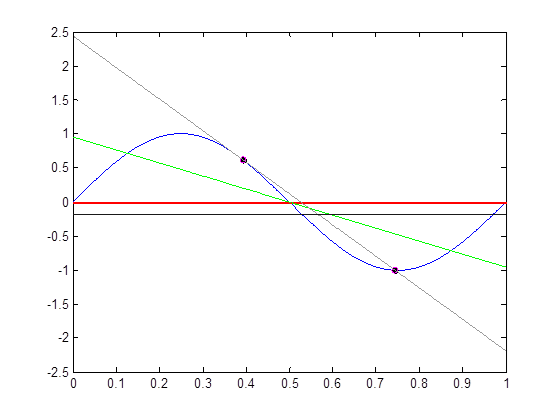
\includegraphics[scale=0.65]{BV_Tradeoff.png}
\caption{사인함수 예제}
\label{Figure 6-3}
\end{figure}

\indent 먼저, 진회색 선과 빨간색 선을 살펴보자. 어떤 사람은, 실제 함수가 이런 상수함수의 형태인데, 관측 오차에 의하여 데이터가 그림처럼 주어졌다고 믿을 수 있다. 그리고 기울어진 직선인 연회색 선과 연두색 선을 살펴보자. 이는 차수가 1인 일차함수 그래프를 이용하여 데이터를 설명하고자 한 것이다. (이러한 형태의 함수를 얻는 방법에는, 간단하게 선형회귀가 있을 것이다.) 만약 우리가, 차수가 1차 이하인 함수만을 사용하여 사인함수를 근사해야 한다면, 위의 4가지 직선 중에서 무엇이 가장 적절한 것일까? 단연 연두색 직선이 사인함수를 가장 잘 표현하고 있다고 할 수 있을 것이다. 먼저, 상수함수인 진회색과 빨간색 선은 $x$값의 변화에 따른 $y$값의 변화를 전혀 반영하지 못하는 함수이고, 연회색 선보다는 연두색 선이 분산(Variance)이 낮음을 관찰할 수 있기 때문이다. 이제, 다음 그림을 살펴보자.
\begin{figure}[ht]
\centering
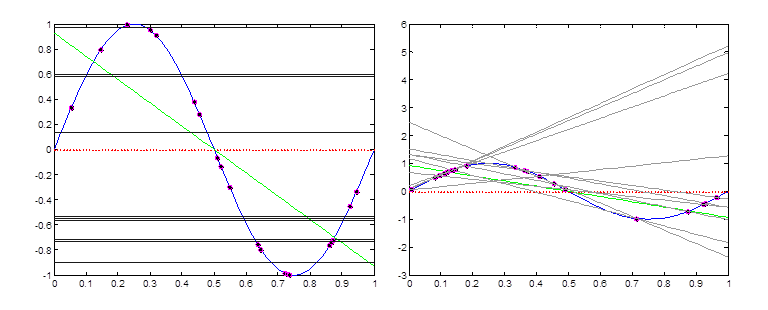
\includegraphics[scale=0.85]{BV_Tradeoff2.png}
\caption{사인함수 예제 2}
\label{Figure 6-4}
\end{figure}

\indent 만약, 주어진 데이터 두 좌표가 모두 $x=0.25$보다 작은 값에서 발생했다면 어떨까? 이를 표현하는 함수는 기울기가 양수인 일차함수가 되었을 것이다. 위에서 오른쪽 그래프를 살펴보자. 여러 가지 회색 선들 중 기울기가 양수인 일차함수를 보면, $x$의 값이 커질수록 실제 사인함수와의 간극은 더 심하게 벌이짐을 볼 수 있다. 반면, 왼쪽 그래프의 함수들처럼 상수함수의 형태이면 $x$의 값이 어디에 있더라도 목표 함수와 크게 차이가 벌어질 수 없다. (항상 2 이하의 차이) 즉, 학습시킨 데이터와 다른 일반적인 데이터가 들어와도 해당 데이터를 적당한 수준에서 설명할 수 있다. 이를 다시 표현하면, 상수함수는 모델의 복잡성이 낮아 현재 주어진 데이터는 잘 설명하지만, 좀 더 일반적인 데이터를 가져와서 테스트 했을 때, 분산이 더 커진다는 것이다. 이것이 바로 분산과 바이어스의 Trade-off 관계이다.

%슬라이드 14
\subsubsection{두 가지 가설의 바이어스와 분산}
이제 다음의 그래프를 살펴보자. 그림에서 각각의 점은 관측된 데이터를 나타내고, 빗금친 영역의 정가운데 위치한 직선은 해당 데이터 셋을 통해 얻은 0차(왼쪽), 1차함수(오른쪽)를 나타낸다. 빗금 영역은 매개변수(Parameter)를 얻는 과정에서 신뢰구간(Confidence Interval)을 구했을 때, 해당 매개 변수의 신뢰구간을 이용하여 그래프를 그리면 색칠된 영역 안에 들어간다는 의미이다. 
\begin{figure}[ht]
\centering
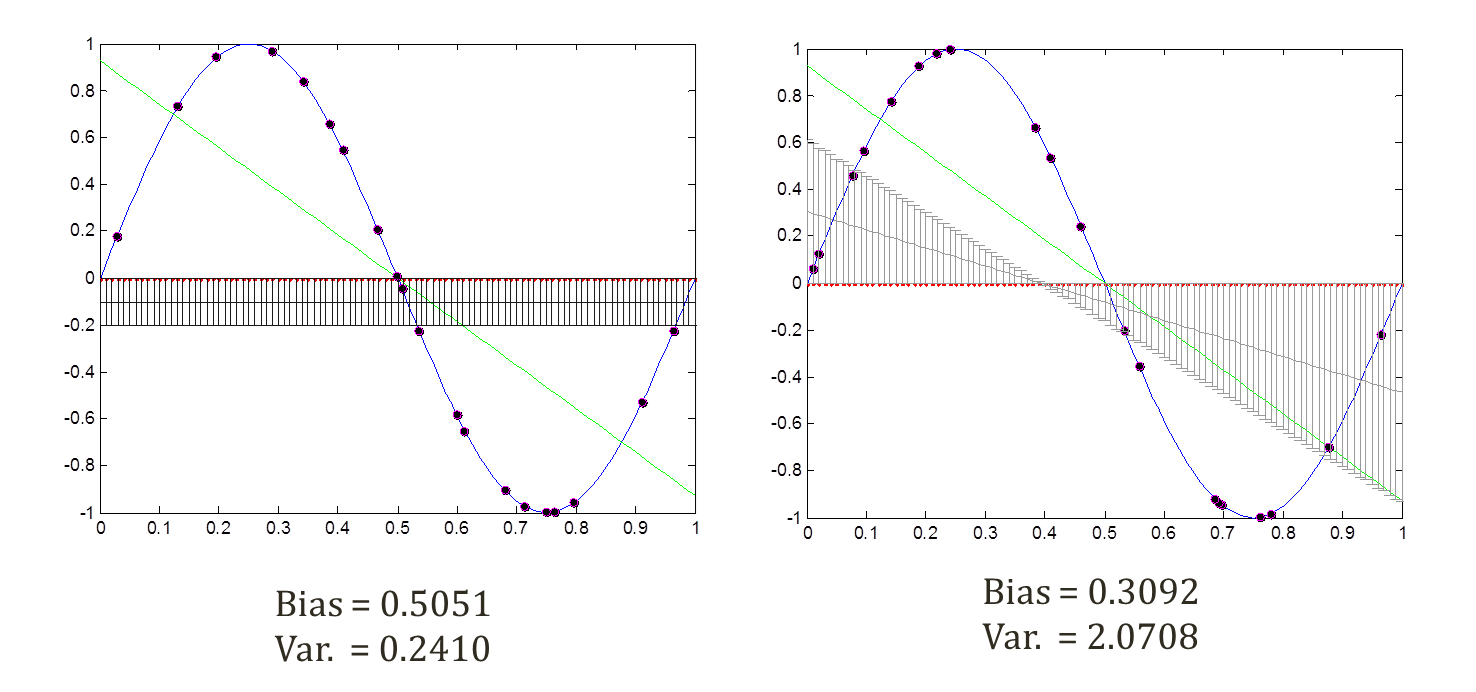
\includegraphics[scale=0.5]{BV_Tradeoff3.png}
\caption{두 가설의 바이어스와 분산}
\label{Figure 6-5}
\end{figure}

\indent 각각의 그래프 아래에 해당 모델의 바이어스와 분산값을 구하여 표시하였다. 이로부터, 오른쪽(1차함수로 fitting)과 같이 더 복잡한 모델은 바이어스가 낮지만 분산이 높고, 왼쪽(상수함수로 fitting)과 같이 간단한 모델은 바이어스가 높고 분산이 낮은 것을 알 수 있다. 따라서, 기계학습에서는 이들 사이의 적절한 균형을 찾는 것이 중요한 과제가 된다.

%슬라이드 15
\subsubsection{오컴의 면도날 (Occam's Razor)}
오컴의 면도날은 14세기 영국의 논리학자인 William of Ockham 에 의해 정립된 원리로써, 흔히 '경제성의 원리(Principle of Economy)'라고도 불린다. 이는 현대 과학이론을 구성하는 데에 핵심적인 역할을 해왔다고 할 수 있다; 수학에서는 Zermelo-Fraenkel 집합론의 10가지 공리 중 단 하나도 다른 공리들로부터 연역될 수 없다는  것(그 외 불필요한 공리는 단 하나도 포함되지 않았다.). 물리학, 화학 등 자연과학에서는 주어진 자연현상을 설명할 때 가장 간단한 가정을 통해 해당 현상을 설명하려 하는 것이 모두 오컴의 면도날을 적용한 것이라고 할 수 있다. \\
\indent 여기서는 바이어스와 분산의 Trade-off 관계를 설명할 때 유용하다고 판단되어 서술한다. 그 내용은 ''비슷한 오차를 보이는(혹은 비슷한 수준의 설명 능력을 가지는) 여러 가지 이론들이 있을 때, 불필요한 가정이 가장 적은 원리를 선택하라''는 것이다. 만약 그림 2 에서 오른쪽 두 개의 가설들이 비슷한 수준의 바이어스를 가진다면, 더 간단한 가설인 가운데 가설을 선택해야 한다는 것이다.

%슬라이드 16
\subsection{Cross Valiation}
앞선 예제에서 우리는 바이어스와 분산 값을 계산하기 위하여 목표 함수가 사인함수라는 것을 가정하고 계산하였다. 또한, 데이터 셋 $D$를 구성할 때는 무한대로 많은 경우의 수만큼 모든 케이스를 다 검사한 것이 아니라, 오직 두 개의 관측 데이터를 포함하는 데이터 셋만 생각했다. 하지만 실제 상황에서 우리는 목표 함수(True function) $f(x)$를 알 수 없다는 것을 상기하자. 즉, 현실에서는 바이어스와 분산을 계산할 방법이 전혀 없다는 것이다. 그리고 데이터 셋 $D$의 샘플링을 무한 번 반복하는 것도 불가능하므로, 이러한 한계를 극복하기 위한 방법이 필요하다. \\
\indent 주어진 데이터 셋 $D$가 있다고 하자. 이 때, '\textbf{N-fold Cross Validation}' 방법은 다음과 같이 진행한다;
\begin{itemize}
\item $D$를 $N$개의 서로 겹치지 않는 부분집합으로 나눈다.
\item 이 중, $(N-1)$개의 부분집합을 임의로 선택하여 학습하는데 사용한다.
\item 나머지 1개의 부분집합을 테스트하는데 사용한다.
\end{itemize}
\begin{figure}[ht]
\centering
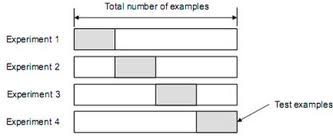
\includegraphics[scale=0.65]{Cross_Validation.png}
\caption{N-fold Cross Validation}
\label{Figure 6-6}
\end{figure}

\indent 데이터 셋 $D$가 매우 크고, 나누는 갯수인 $N$ 역시 매우 크다면, Cross Validation은 마치 데이터의 샘플링을 무한 번 반복하는 것과 비슷한 효과를 가질 수 있다. (하지만, 실제로는 오직 단 한 번의 샘플링만 이루어졌고, 제한된 데이터 셋 $D$ 안에서 이들을 임의로 나누어 마치 많은 수의 샘플링이 이루어진 것처럼 흉내내는 것이다.)  \\
\indent 그렇다면 최대 몇 번까지 샘플링을 하는 것처럼 설정할 수 있을까? 당연하게도, 데이터 셋 $D$의 관측값의 갯수만큼 가능할 것이다. 1개의 테스트 데이터만 남기고 나머지는 모두 학습하는 데에 사용하는 Singleton 부분집합들로 만드는 것이다. 이를 'Leave One Out Cross Validation(LOOCV)' 방법이라 부르는데, 이는 단지 N-fold Cross Validation의 극단적인 예시에 불과하다.

%슬라이드 17, 18
\subsection{기계학습에서의 성능 척도(Performance Measure)}
앞서 말한대로, 우리는 실제 함수(목표 함수, target function)를 알 수 없기 때문에, 바이어스나 분산을 이용하여 알고리즘의 성능을 측정할 수는 없다. 특히, 분류 작업(Classification)을 하는 기계학습 알고리즘은 상황에 따라 다른 종류의 성능 평가지표를 사용해야 하는데, 먼저 다음의 $2 \times 2$ Contingency Table(Confusion Matrix)을 살펴보자.
\begin{figure}[ht]
\centering
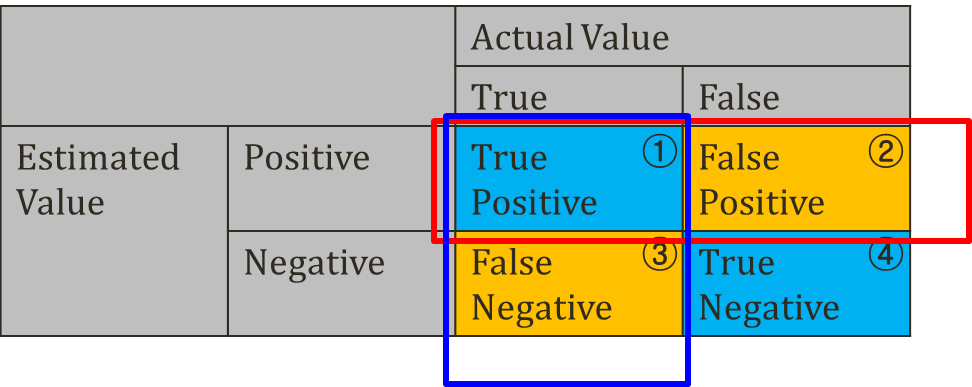
\includegraphics[scale=0.65]{Contingency_Table.png}
\caption{실제 값과, 추정 값에 따른 참/거짓 표}
\label{Figure 6-7}
\end{figure}

\indent 표에서 알 수 있듯이, 각 데이터는 2가지 값만 가질 수 있는 이산적인(Discrete) 경우이다. 데이터의 실제 값이 True 혹은 False로 표시되었고, 우리가 이 데이터를 분류한 결과를 Positive, Negative로 나누었다. 분류한 결과가 맞으면 표의 (1)$\sim$(4)에서 True로 시작하는 부분이고(하늘색), 분류한 결과가 틀렸을 때는 False로 시작하는 영역에(귤색) 해당한다. (1) True Positive 는 말그대로 Positve로 분류했고 이 결과가 옳을 때, (4) True Negative 는 Negative로 분류했고 이 결과가 맞을 때를 의미한다. (2) False Positive, (3) False Negative 는 각각 Positive, Negative로 분류했으나 실제 값이 이와 달라서 틀린 경우를 의미한다. 이 표로부터 다양한 종류의 성능 평가지표(Performance Measure)를 정의할 수 있다;
\begin{itemize}
\item Accuracy = $\dfrac{(TP + TN)}{(TP + FP + FN + TN)}$
\item Precision = $\dfrac{TP}{(TP + FP)}$
\item Recall = $\dfrac{TP}{(TP + FN)}$
\item F-measure = Precision 과 Recall 의 조화평균
\item ROC Curve
\end{itemize}

\indent 다음의 두 가지 경우를 생각해보자; 분류 작업을 수행하는 기계학습 알고리즘을 만드려고 하는데, 이를 (a) 스팸메일 필터링을 목적으로 하는 경우, (b) 고객을 관리하는 목적으로 하는 경우 중요하게 생각하는 Performance Measure가 다를 수 있다. \\
\indent 먼저, (a) 의 경우를 생각해보자. 이 예시에서 표의 (1) 영역은 스팸메일이 제대로 인식된 경우, (2) 영역은 업무메일이 스팸메일로 잘못 분류된 경우, (3) 은 실제 스팸메일이 받은 메일함에 있는 경우, (4) 는 업무메일이 정상적으로 받은 메일함에 있는 경우이다. 이 때는 단연 안정성이 최우선이다. 다시 말하면, 광고메일이 가끔 스팸메일로 분류되지 않더라도 소수의 메일은 사용자가 직접 스팸처리를 할 수도 있다. 반면, 중요한 메일을 알고리즘이 잘못 판단하여 스팸메일로 처리하면 업무상 심각한 지장이 초래되므로 이를 반드시 피해야 한다. 즉, (2) False Positive 영역을 최대한 낮춘 알고리즘을 만들어야 한다. 따라서, (a)의 경우에는 \textbf{Precision}을 중요시하게(precision이 높은 것을 추구) 된다. \\
\indent (b)의 경우에는 어떨까? 여기서 CRM은 구체적으로, 잠재적인 VVIP 고객을 찾는 업무라고 하자. 잠재적 VVIP 고객으로 분류되면, 기업은 해당 고객을 대상으로 집중적인 마케팅 투자를 통해 수익을 극대화할 수 있을 것이다. (1) 영역은 실제로 VVIP가 될 고객을 잘 찾아낸 경우, (2) 는 고객이 VVIP 등급이 되지 않지만 잠재적 VVIP로 분류된 경우, (3) 은 VVIP가 될 수 있는 고객이지만 회사에서 이를 알아보지 못한 경우, (4) 는 VVIP가 될 가능성이 없고 이를 잘 선별한 경우가 되겠다. 기업 입장에서 조금이라도 더 많은 수익을 거두기 위해서는 VVIP 등급이 될 가능성이 높은 고객을 조금이라도 더 찾아야 한다. 즉, (3) 영역에 해당하는 사람의 수를 최소화해야 한다. 따라서, (b)의 경우에는 \textbf{Recall}을 중요시하게(recall이 높은 것을 추구) 된다. \\
\indent 위의 예시들을 완벽하게 이해했다면 다음으로 넘어가도록 하자. 하나의 예시를 더 들자면, 공항에서 테러리스트를 찾아내는 작업을 들 수 있겠다. 이 때는 어떤 평가지표가 중요할까? 테러리스트가 테러를 위해 공항을 통과하려 한다면, 무슨 수를 쓰더라도 그를 잡아야 하므로 (3)의 영역이 중요하고, 따라서 \textbf{Recall}이 높도록 검문을 실시할 것이다.

%슬라이드 19
\subsubsection{F-Measure}
Precision 과 Recall 모두 실생활에서 이용되고 있지만, 어느 하나만 중요하게 생각할 수는 없다. 스팸메일 예제에서, precision을 높이기 위해 무조건 스팸이 없다고 분류한다면, 중요한 메일을 놓치지 않을 수는 있겠지만 받은 메일함이 불필요한 것들로 가득찰 수 있다. 그리고 CRM 예시에서는, 모든 고객을 잠재적 VVIP 로 분류하면, 이들을 관리하는 데에 너무 많은 비용이 소모될 수 있다. 따라서, 이 두 가지 지표를 모두 아우르는 평가 지표가 필요한데, 이러한 F-measure 가 실생활에서 가장 많이 사용되는 성능의 척도이다. 일반적인 정의는 다음과 같다;
\begin{equation}
F_{b}-Measure := \dfrac{(1+b^{2})*(Precision*Recall)}{b^{2}*Precision + Recall} \tag{6-11}
\end{equation}

\indent $b=1$ 이면, 일반적으로 많이 사용되는 F-measure 이고, 이는 precision과 recall의 조화평균과 같다. $b=$0.5 or 2 도 많이 사용되는데, $F_{0.5}$는 precision 에 더 큰 비중을 둔 지표이고, $F_{2}$는 recall 에 더 큰 비중을 둔다. 앞의 예시를 다시 살펴보면, (a)의 스팸메일 알고리즘은 $F_{0.5}$를, (b)의 CRM 알고리즘은 $F_{2}$를 성능 지표로 사용하면 될 것이다.

%슬라이드 20
\section{모델 정규화(Model Regularization)}

%슬라이드 21
\subsection{정규화(Regularization)의 의미}
이 장의 앞선 부분에서 그림 4의 오른쪽 그래프를 다시 살펴보자. 사인함수를 Fitting 하려 하는데, 오직 두 개의 점만 데이터로 주어졌을 때 어떤 데이터가 주어지냐에 따라 선형회귀의 결과가 아주 다르게 나타날 수 있음을 상기하자. 특히, 왼쪽에 치우진 점들만 주어지면 그래프는 양의 기울기를 가지게 되는데, 이 때는 미래에 들어올 테스트 데이터에 대해 분산 값이 아주 크게 나타났었다. \\
\indent 그렇다면 분산을 줄일 수 있는 방법에는 어떤 것들이 있을까? 모델의 복잡성과 데이터의 일반성 사이에는 Trade-off 관계가 있다는 것을 기억하면, 한 가지 답을 알 수 있다. 바로 모델의 복잡성을 낮추는 것이다. 하지만, 너무 단순한 모델을 사용하면, 바이어스를 허용하게 되므로 그렇게 좋은 방법은 아니다. 이 장에서 공부할 정규화는 복잡한 모델은 그대로 두면서, 분산을 줄이는 기술이라 할 수 있다. 복잡성을 유지하므로, 바이어스는 비교적 낮은 수준으로 유지될 것이다. \\
\indent 정규화의 핵심은 완벽한 Fitting을 포기한다는 것이다. 즉, 주어진 데이터를 가장 완벽하게 설명하는 매개변수를 학습하는 것보다는, 이를 다소 포기하더라도 이후에 주어질 일반적인 데이터를 충분히 잘 설명할 수 있도록 분산을 줄이는 것이다. 이 방법은 모델이 주어진 데이터에 다소 '둔감'해지도록 만든다. 사인함수 예제에서 정규화를 적용하면 어떤 두 점이 주어졌을 때, 단순히 그 점들을 잇는 직선을 그리지 않게 된다. 그 결과, 당연히 학습의 정확도는 떨어질 것이다.

%슬라이드 22
\subsubsection{정규화(Regularization)의 엄밀한 정의}
정규화를 수학적으로 엄밀하게 정의하기 위해서, (선형 혹은 다항) 회귀에서 어떻게 사용되는지 살펴보자.
\begin{equation}
E(w) = \frac{1}{2}\sum_{n=0}^{N}\left(train_{n} - g(x_{n}, w) \right)^{2} + \lambda \|w\|^{2} \tag{6-12}
\end{equation}

\indent 위의 식을 이해하기 위해서, 2단원에서 선형회귀를 다루었던 부분을 떠올리자. 괄호 안의 식을 최소화시키는(argument minimum) 매개변수 $\hat{\theta}$ 을 찾기 위해 해당 식을 미분하여 미분계수가 0이 되는 지점을 찾았다. 여기서 최소화시키고자 했던 최초의 식을 Cost Function 혹은 Loss Function이라 부른다. 식 6-12 에서 마지막 항을 제외한 앞 부분은 이러한 Loss Function의 형태이다. 주어진 데이터인 $train_{n}$에서 회귀의 결과로 추정한 값 $g(x_{n}, w)$을 뺀 것의 제곱, 즉, 제곱 오차의 합인(Sum of Squared Errors) 것이다. 선형회귀에서는 식 6-12 의 마지막 항 없이, Loss Function을 최소화하는 매개변수의 값을 구했다. 하지만 마지막 항인 $\lambda \|w\|^{2}$(정규화 항, Regularization Term)을 더해주면, Loss Function을 최소화하는 매개변수의 값도 달라질 것이다. \\
\indent 그렇다면 정규화 항은 어떤 역할을 하는 것일까? 이는 해당 항을 어떤 형태로 더해주느냐에 따라 조금씩 달라지지만, 흔히 많이 사용되는 1차 절댓값, 2차 절댓값을 사용하는 정규화를 각각 L1 정규화(Lasso 정규화), L2 정규화(Ridge 정규화) 이라 부른다.
\begin{figure}[ht]
\centering
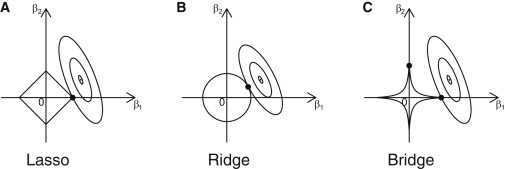
\includegraphics[scale=0.8]{L1_L2_Regularization.png}
\caption{정규화의 여러 가지 형태}
\label{Figure 6-8}
\end{figure}

\indent 위의 그림은 3가지 종류의 정규화 형태를 나타낸다. 세 그래프에서 최소화시키고자 하는 제곱 오차는 제 1사분면에 위치한 타원 형태로 나타나고, 정규화 항은 원점을 중심으로 대칭인 도형이다. Loss Function을 최소화시키려면, 두 그래프가 서로 접하거나, 접하는 것이 불가능할 경우엔 가장 바깥쪽에서 서로 만나는 경우가 될 것이다. (고등학교 수학 문제에서 최대/최소값 문제를 상기하자.)

%슬라이드 23
\subsection{선형회귀에서의 정규화}
이번에는 Ridge 정규화를 이용하여 선형회귀를 다루어 보자. Loss Function은 다음과 같이 정의될 수 있다;
\begin{equation}
E(w) = \frac{1}{2}\sum_{n=0}^{N}\left(train_{n} - g(x_{n}, w) \right)^{2} + \frac{\lambda}{2} \|w\|^{2} \tag{6-13}
\end{equation}

선형회귀를 이용할 것이므로, 데이터를 통해 학습된 함수 $g$는 선형함수가 될 것이다. 2단원에서와 마찬가지로, 최소화하고자 하는 Loss Function의 미분계수가 0이 되는 지점을 찾아보자;
\begin{align}
\frac{d}{dw}E(w) &=\frac{d}{dw}\left(\frac{1}{2}\| train - Xw \|^{2} + \frac{\lambda}{2}\|w \|^{2} \right) \tag{6-14}\\
&=\frac{d}{dw}\left(\frac{1}{2}(train - Xw)^{T}(train - Xw) + \frac{\lambda}{2}w^{T}w \right) \tag{6-15}\\
&=\frac{d}{dw}\left(\frac{1}{2}(train^{T}train - 2X^{T}w*train + X^{T}X*w^{T}w)+\frac{\lambda}{2}w^{T}w \right) \tag{6-16}\\
&=\frac{d}{dw}\left(train^{T}train - X^{T}w*train + \frac{1}{2}X^{T}X*w^{T}w + \frac{\lambda}{2}w^{T}w \right) \tag{6-17}\\
&=-X^{T}*train + X^{T}Xw + \lambda w \tag{6-18}\\
&=0 \tag{6-19}
\end{align}

\indent Loss Function을 최소화하는 매개변수의 값을 찾아야 하므로 $E(w)$를 $w$에 대해 미분하여 식을 전개한다. 벡터의 Norm의 정의에 의해 식 6-15 와 같이 나타낼 수 있고, 이를 전개하여 계산하면 6-16, 6-17 로 표현된다. 행렬 미분을 실시하면, 6-18 의 결과를 손쉽게 얻을 수 있다. 최종 결과를 얻기 위하여 계속 진행하자;
\begin{align}
&-X^{T}*train + X^{T}Xw + \lambda Iw = 0 \tag{6-20}\\
&\to -X^{T}*train + (X^{T}X + \lambda I)w = 0 \tag{6-21}\\
&\to (X^{T}X + \lambda I)w = X^{T}*train \tag{6-22}\\
&\: \therefore w = (X^{T}X + \lambda I)^{-1}X^{T}*train \tag{6-23}
\end{align}

\indent 벡터로 표현된 방정식이므로, 6-20 과 같이 Identity 행렬을 곱해주는 것은 식을 변화시키지 않는다. 적절히 이항하여 식을 정리하면, 최종적으로 6-23 처럼 닫힌 형태(Closed Form)의 해 $w$를 구할 수 있다. 2단원에서 다루었던 선형회귀와 어떻게 다른가? 괄호 안의 $\lambda I$ 부분이 더해진 것이 앞서 보았던 선형회귀의 결과와 다른 점이다. 여기서 $\lambda$는 정규화를 통해 얼마나 강력하게 Loss Function을 통제할 것인지 결정하는 상수로서, 그 값은 우리가 임의로 설정할 수 있다. $\lambda$의 값이 크면, 매개변수 벡터의 크기가 조금만 커져도 Loss Function의 값이 크게 증가하므로, 선형회귀의 결과인 $w$ 벡터는 크기가 비교적 작을 것이다. 반면, $\lambda$ 값을 작게 설정하면, 정규화 항이 Loss Function에 크게 영향을 미치지 않으므로 $w$ 벡터의 크기가 비교적 크게 나타날 것이다.

%슬라이드 24
\subsubsection{정규화의 효과}
\begin{figure}[ht]
\centering
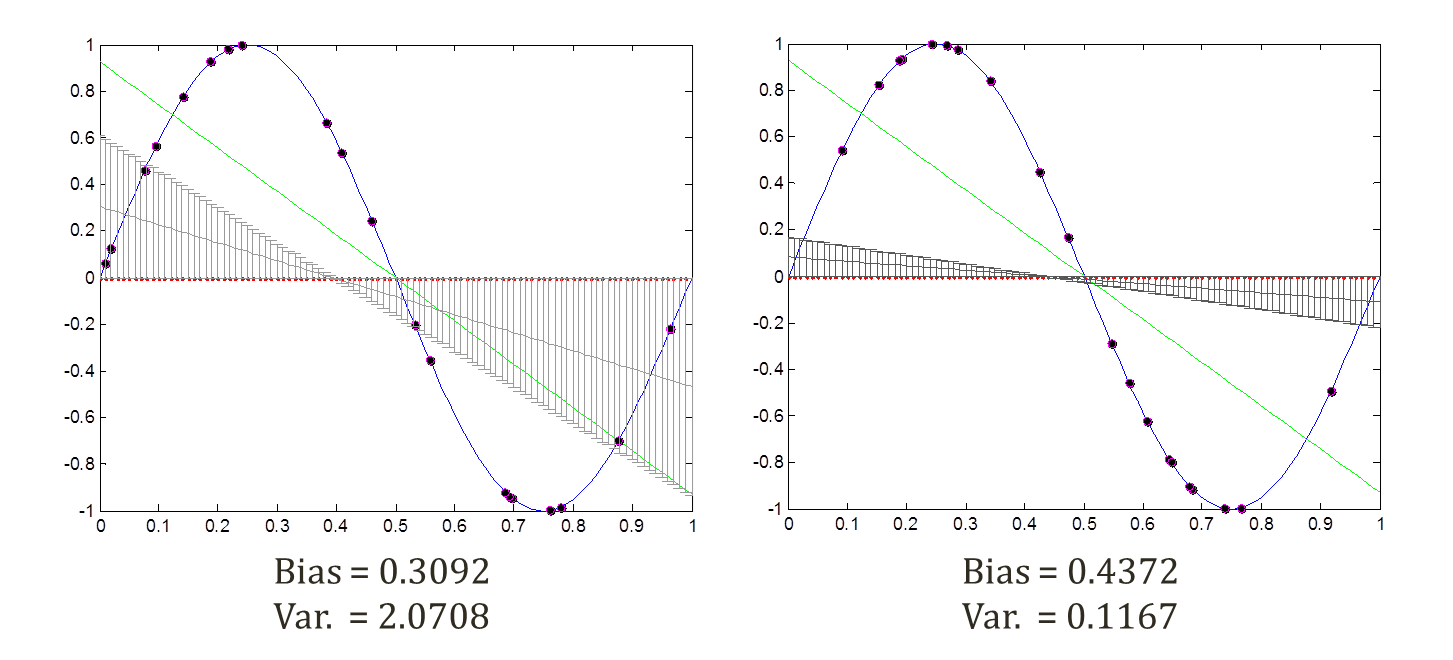
\includegraphics[scale=0.5]{Regularization_Effect.png}
\caption{사인함수 Fitting 예제에서 정규화의 효과 비교}
\label{Figure 6-9}
\end{figure}

\indent 왼쪽의 그래프는 앞서 사인함수를 Fitting하는 예제에서 정규화를 사용하지 않았을 때, 주어진 데이터 분포를 변화시키며 평균 매개변수를 추정, 그리고 이 매개변수의 신뢰구간(Confidence Interval)을 이용하여 그림과 같이 나타낸 것이다. 연두색은 (주어진 데이터만을 이용한 것이 아닌) 실제 목표함수에서 가능한 모든 데이터 셋을 이용하여 학습한 함수의 기댓값에 해당한다. 이 때의 바이어스와 분산은 아래의 값과 같다. 오른쪽 그래프는 다른 데이터 분포를 이용하긴 했지만, 정규화 기법을 사용하여($\lambda = 1$) 평균 매개변수 및 신뢰구간을 구하여 나타낸 것이다. 바이어스와 분산 값은 아래에 나타나 있다. \\
\indent 두 그래프를 비교하면, 정규화를 사용했을 때, 분산이 줄어든 것을 육안으로 확인할 수 있다. 이는 분산값을 통해서도 알 수 있다. 모델의 복잡성이 변하지 않으면서 주어진 데이터에 '둔감하게' 반응한 것이다. 또한 정규화를 사용했을 때, 바이어스의 값이 증가했는데, 앞 부분에서 설명했듯이 완벽한 Fitting을 포기하며 앞으로 올 일반적인 데이터에 대해 더 잘 작동하도록 했기 때문이다.

%슬라이드 25
\subsubsection{정규화의 최적화}
\begin{figure}[ht]
\centering
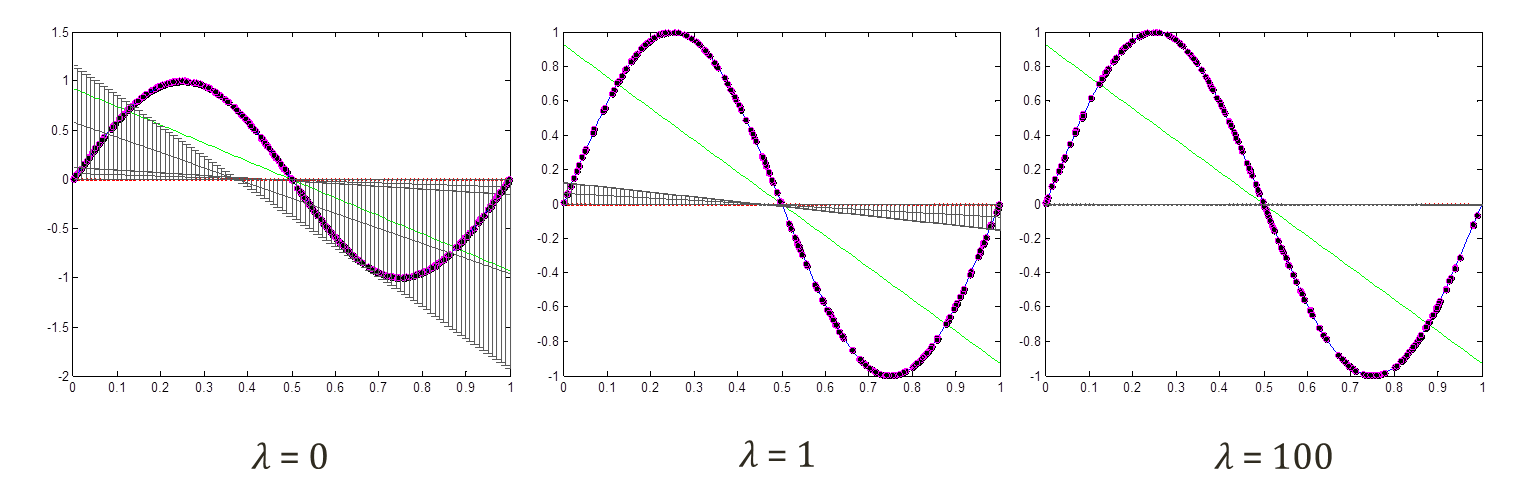
\includegraphics[scale=0.5]{Optimizing_Regularization.png}
\caption{$\lambda$ 값을 변화시켰을 때 정규화의 효과}
\label{Figure 6-10}
\end{figure}

\indent 위의 그림에서, 왼쪽에서 오른쪽으로 갈수록 $\lambda$의 값을 증가시키며 정규화 항이 Loss Function을 더욱 강력하게 통제하도록 설정하였다. $\lambda$ 값이 너무 작으면, 정규화를 적용시키지 않은 모델처럼 작동하게 되며, 높은 분산값을 가지게 된다. 즉, 일반적인 데이터에 대해 잘 작동하지 않을 수 있다. \\
\indent 반면 $\lambda$ 값을 너무 크게 설정하면, 매개변수 벡터의 값이 단 하나라도 0이 아닌 값을 가질 때, 정규화 항이 급격하게 커지면서 Loss Function 의 값을 증가시킨다. 우리는 Loss Function을 최소화시키는 것이 목적이므로, 이는 바람직하지 않다. 즉, $\lambda$ 값이 클 때, 매개변수는 거의 0에 가까워지며 이는 곧 가장 단순한 모델인 상수함수의 형태로 수렴함을 의미한다. 그렇다면, 적절한 수준의 $\lambda$ 값은 어떻게 찾을 수 있을까? 수학적인 방법이 있지만, 우선은 시행착오를 통해 최적화된 값을 찾는다고 알아두자. 기계학습 알고리즘은 모델을 찾는 것에서 끝이 아니라, 매개변수의 최적화부터 메타 매개변수인 $\lambda$의 최적화까지 많은 시도를 통해 적절한 변수 값을 찾는 고단한 여정이라고 할 수 있겠다.

%슬라이드 26
\subsection{로지스틱 회귀에서의 정규화}
선형회귀에서 그치지 않고, 이를 로지스틱 회귀에도 적용할 수 있을까? 당연히 가능하다. 지난 4단원에서 배웠던 로지스틱 회귀의 유도 과정에서 최적화된 매개변수 $\hat{\theta}$는 다음의 식을 만족했던 것을 상기하자;
\begin{equation}
\hat{\theta} = argmax_{\theta}\sum_{1 \leq i \leq N}log(P(Y_{i} \mid X_{i}; \theta)) \tag{6-24}
\end{equation}

\indent 우리는 이 식에 정규화 항 $L_{1}: R(\theta) = \| \theta \|_{1} = \sum_{i=1}^{N}\mid \theta_{i} \mid$ 또는 \\ $L_{2}: R(\theta) = \| \theta \|_{2}^{2} = \sum_{i=1}^{N}\theta_{i}^{2}$ 를 빼주어 Loss Function 을 수정할 것이다. 여기서는 선형회귀와 달리 argument minimum이 아닌 argument maximum의 형태이므로 (Conditional Maximum Likelihood Estimator; CMLE, 조건부 Likelihood 를 최대화시키는 Estimator) Loss Function이 사실은 Gain Function과 같이 작용하게 된다. 즉, 함수값을 최대한 증가시켜야 하는데, 정규화 항을 빼줌으로써 해당 함수를 통제해주는 것이다. \\
\indent 지난 4단원에서 이 MCLE 값을 구하기 위해, 경사법(Gradient Ascent)이라는 Numerical 한 방법을 사용했던 것을 기억하자. 이는 $\hat{\theta}$의 방정식을 이용하여 닫힌 형태의 해를 구할 수 없었기 때문이다. 여기서도 마찬가지로 닫힌 형태의 해를 구할 수 없다. 따라서 경사법이나 다른 Numerical 한 도구를 이용하여 해를 근사해야 한다. 엄밀한 유도과정은 독자분들께 과제로 남긴다.

%슬라이드 27
\subsection{SVM에서의 정규화}
Support Vector Machine에서는 Soft Margin을 적용한 시점에 이미 정규화의 개념을 사용하고 있었다! 결정 경계(Decision Boundary)를 구하는 과정에서 사용한 상수 $C = \frac{1}{2\lambda n}$를 상기하자. 우리는 앞 단원에서 $C$의 값을 변화시킬 때 결정 경계가 어떻게 변하는지도 살펴보았다. 따라서, 독자는 SVM이 단순히 Hinge Loss 함수에 정규화 기법을 적용한 특수한 예에 불과하다는 것을 알 수 있을 것이다.
\begin{figure}[ht]
\centering
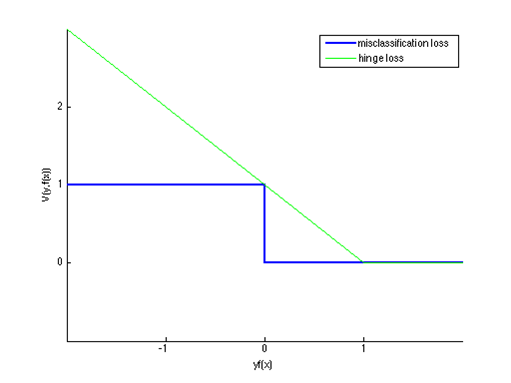
\includegraphics[scale=0.7]{SVM.png}
\caption{Hinge Loss 함수의 그래프}
\label{Figure 6-11}
\end{figure}

\indent 다음의 방정식들을 살펴보며 SVM에서 다루었던 내용을 다시 떠올리자.
\begin{align}
f &= argmin_{f \in \mathcal{H}} \left\{ \dfrac{1}{n}\sum_{i=1}^{n}V(y_{i}, f(x_{i})) + \lambda \| f \|_{\mathcal{H}}^{2} \right\} \tag{6-25}\\
&= argmin_{f \in \mathcal{H}} \left\{ \dfrac{1}{n}\sum_{i=1}^{n}(1-yf(x))_{+} + \lambda \| f \|_{\mathcal{H}}^{2} \right\} \tag{6-26}\\
&= argmin_{f \in \mathcal{H}} \left\{ C\sum_{i=1}^{n}(1-yf(x))_{+} + \frac{1}{2} \| f \|_{\mathcal{H}}^{2} \right\} \tag{6-27}
\end{align}
where $V(y_{i}, f(x_{i})) = (1-yf(x))_{+}$,   $(s)_{+} = max(s,0)$,   $C=\frac{1}{2 \lambda n}$\\

%슬라이드28
\section*{Acknowledgement}
This slideset is greatly influenced by
\begin{itemize}
\item Professor Eric Xing at CMU
\end{itemize}

%보충설명 APPENDIX
\section*{Appendix}
\subsection*{$L_{p}$-Norm in Vector Spaces}
정규화의 종류에서 앞에 $L_{1}$, $L_{2}$ 등을 붙이는 것은 수학에서의 $L_{p}$-Norm 을 가져온 것이다. $L_{p}$-Norm은 무엇일까? 우선, Vector Space(벡터 공간)에서 정의되는 가장 일반적인 Norm 부터 정의하자; \\
\indent Vector Space $V$가 복소수 Field의 Subfield인 $F$에서 정의되었을 때, Norm 함수 $p: V \to \mathds{R}$는 다음의 성질을 만족시키는 함수로 정의한다.\\ $\forall a \in F, \: \forall \textbf{u}, \textbf{v} \in V$, \begin{itemize}\itemsep0pt
\item[] 1. $p(a\textbf{v}) =\: \mid a \mid \: p(\textbf{v})$
\item[] 2. $p(\textbf{u} + \textbf{v}) \leq \: p(\textbf{u}) + p(\textbf{v})$
\item[] 3. $p(\textbf{v})=0 \implies \textbf{v}=\textbf{0}$
\end{itemize}

\indent 특히, $L_{p}$-Norm은 다음과 같이 정의한다; $\| \textbf{x} \|_{p} := \left( \sum_{i=1}^{n}\mid x_{i} \mid^{p} \right)^{1/p}$. $p=1$일 때, 즉 $L_{1}$-Norm 은 Taxicab-norm 이라고도 부른다. 왜냐하면, 식의 형태가 마치 택시가 원점으로부터 출발하여 해당 좌표까지 직각의 도로를 따라 이동하는 거리와 같기 때문이다. $L_{2}$-Norm 은 우리가 고등학교 시절부터 사용했던 Euclidean-norm 이다. $p$의 값에 따라 다양하고 흥미로운 종류의 Norm 이 존재하지만, 더 궁금한 독자는 수학 서적을 참고하길 바란다.
\end{document}
%--------------------------------------------------------------------------------------------------
%알고리즘(pseudo-code) 넣기
\indent\rule{10cm}{0.4pt} \\
\begin{algorithm}[H]
	\SetAlgoLined
	\KwData{Training Dataset}
	\KwResult{Find the Correct Hypothesis}
	Initialize $h = h_{0}$
	\For{instance $x$ in $D$}{
		\eIf{$x$ is positive}{
			\For{Feature $f$ in $O$}{
				\eIf{$f_{i}$ in $h == f_{i}$ in $x$}{
					Do Nothing;
				}{
					$f_{i}$ in $h = f_{i}$ in $h \cup f_{i}$ in $x$
				}
			}
		}{}
	}
\end{algorithm}

\indent \rule{10cm}{0.4pt} \\
%--------------------------------------------------------------------------------------------------